\hypertarget{patStats_8h}{
\section{pat\-Stats.h File Reference}
\label{patStats_8h}\index{patStats.h@{patStats.h}}
}
{\tt \#include $<$stdio.h$>$}\par
{\tt \#include $<$stdlib.h$>$}\par
{\tt \#include $<$string.h$>$}\par
{\tt \#include $<$errno.h$>$}\par
{\tt \#include \char`\"{}bit\-Set.h\char`\"{}}\par
{\tt \#include \char`\"{}convll.h\char`\"{}}\par
{\tt \#include $<$time.h$>$}\par


Include dependency graph for pat\-Stats.h:\begin{figure}[H]
\begin{center}
\leavevmode
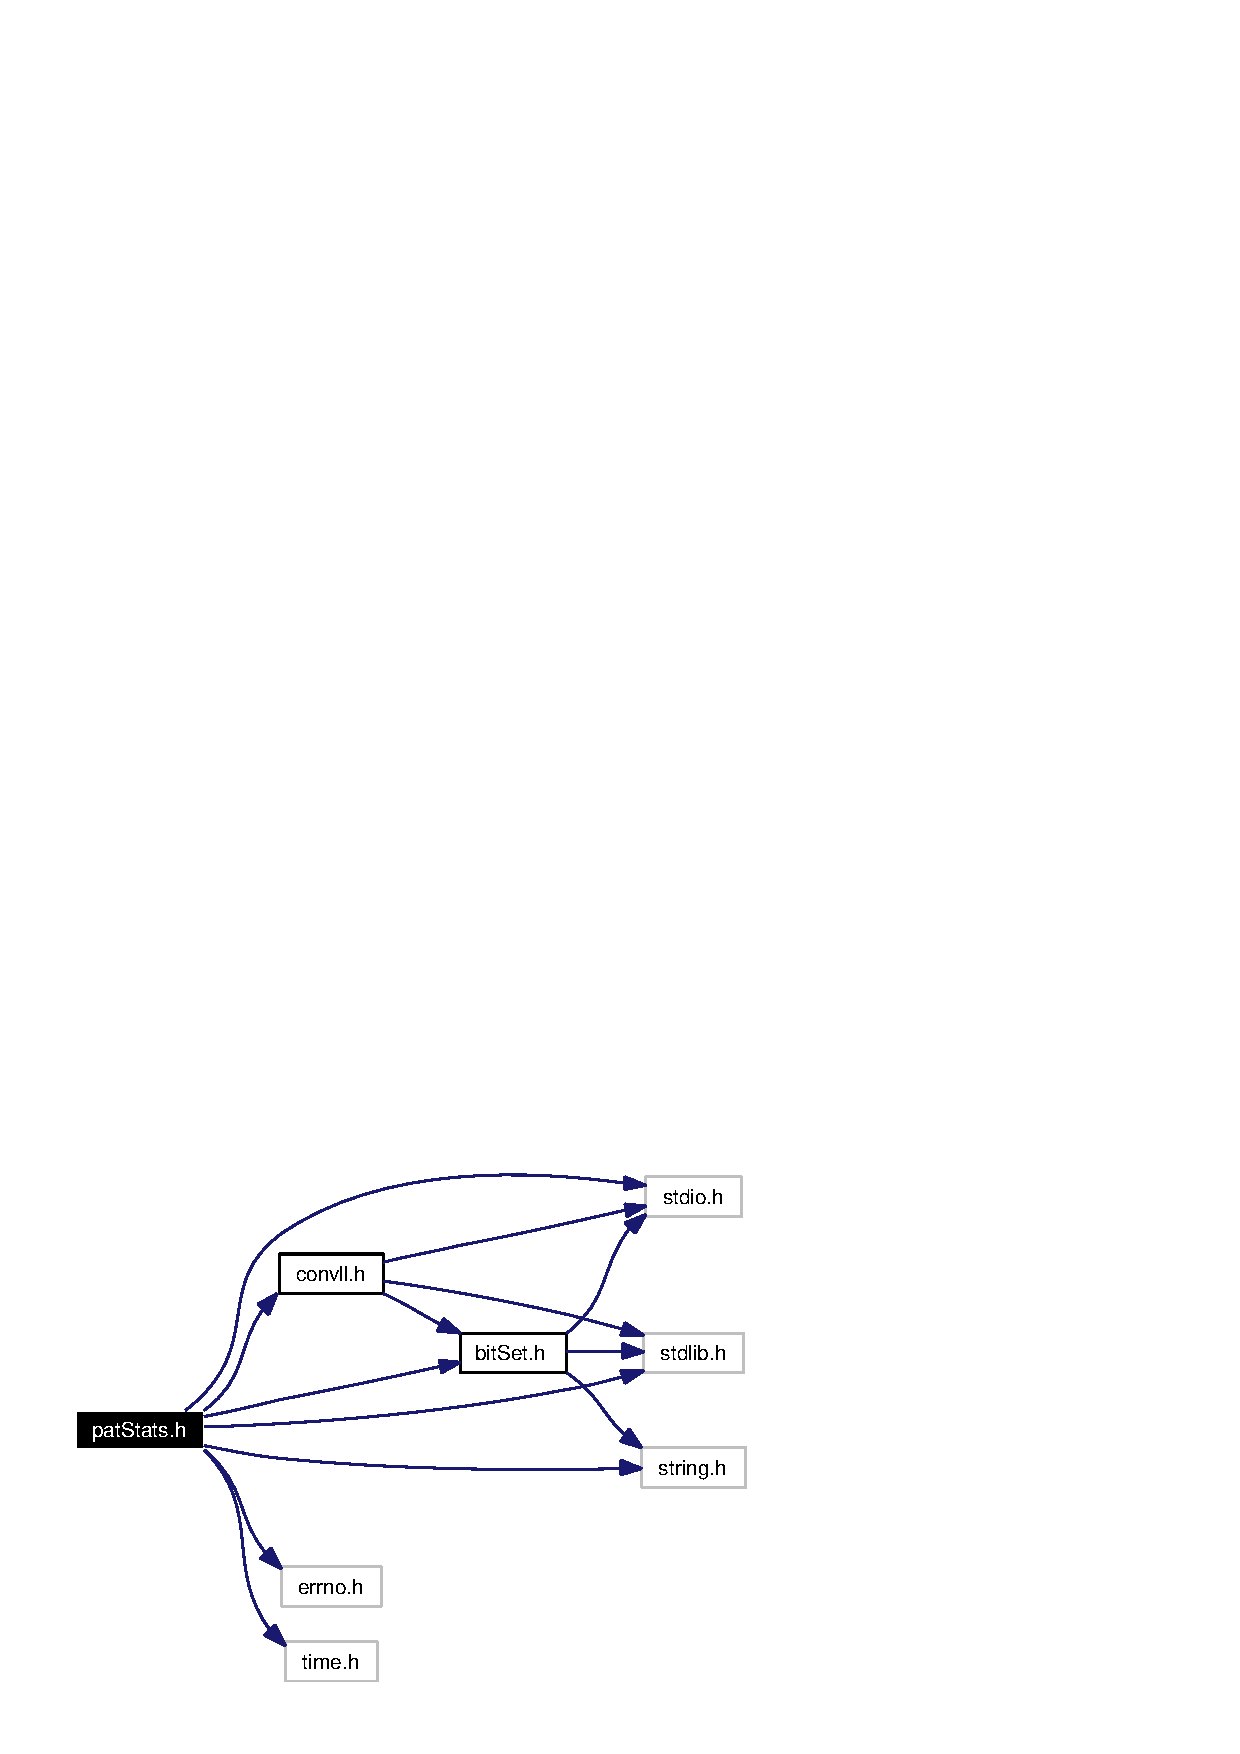
\includegraphics[width=179pt]{patStats_8h__incl}
\end{center}
\end{figure}


This graph shows which files directly or indirectly include this file:\begin{figure}[H]
\begin{center}
\leavevmode
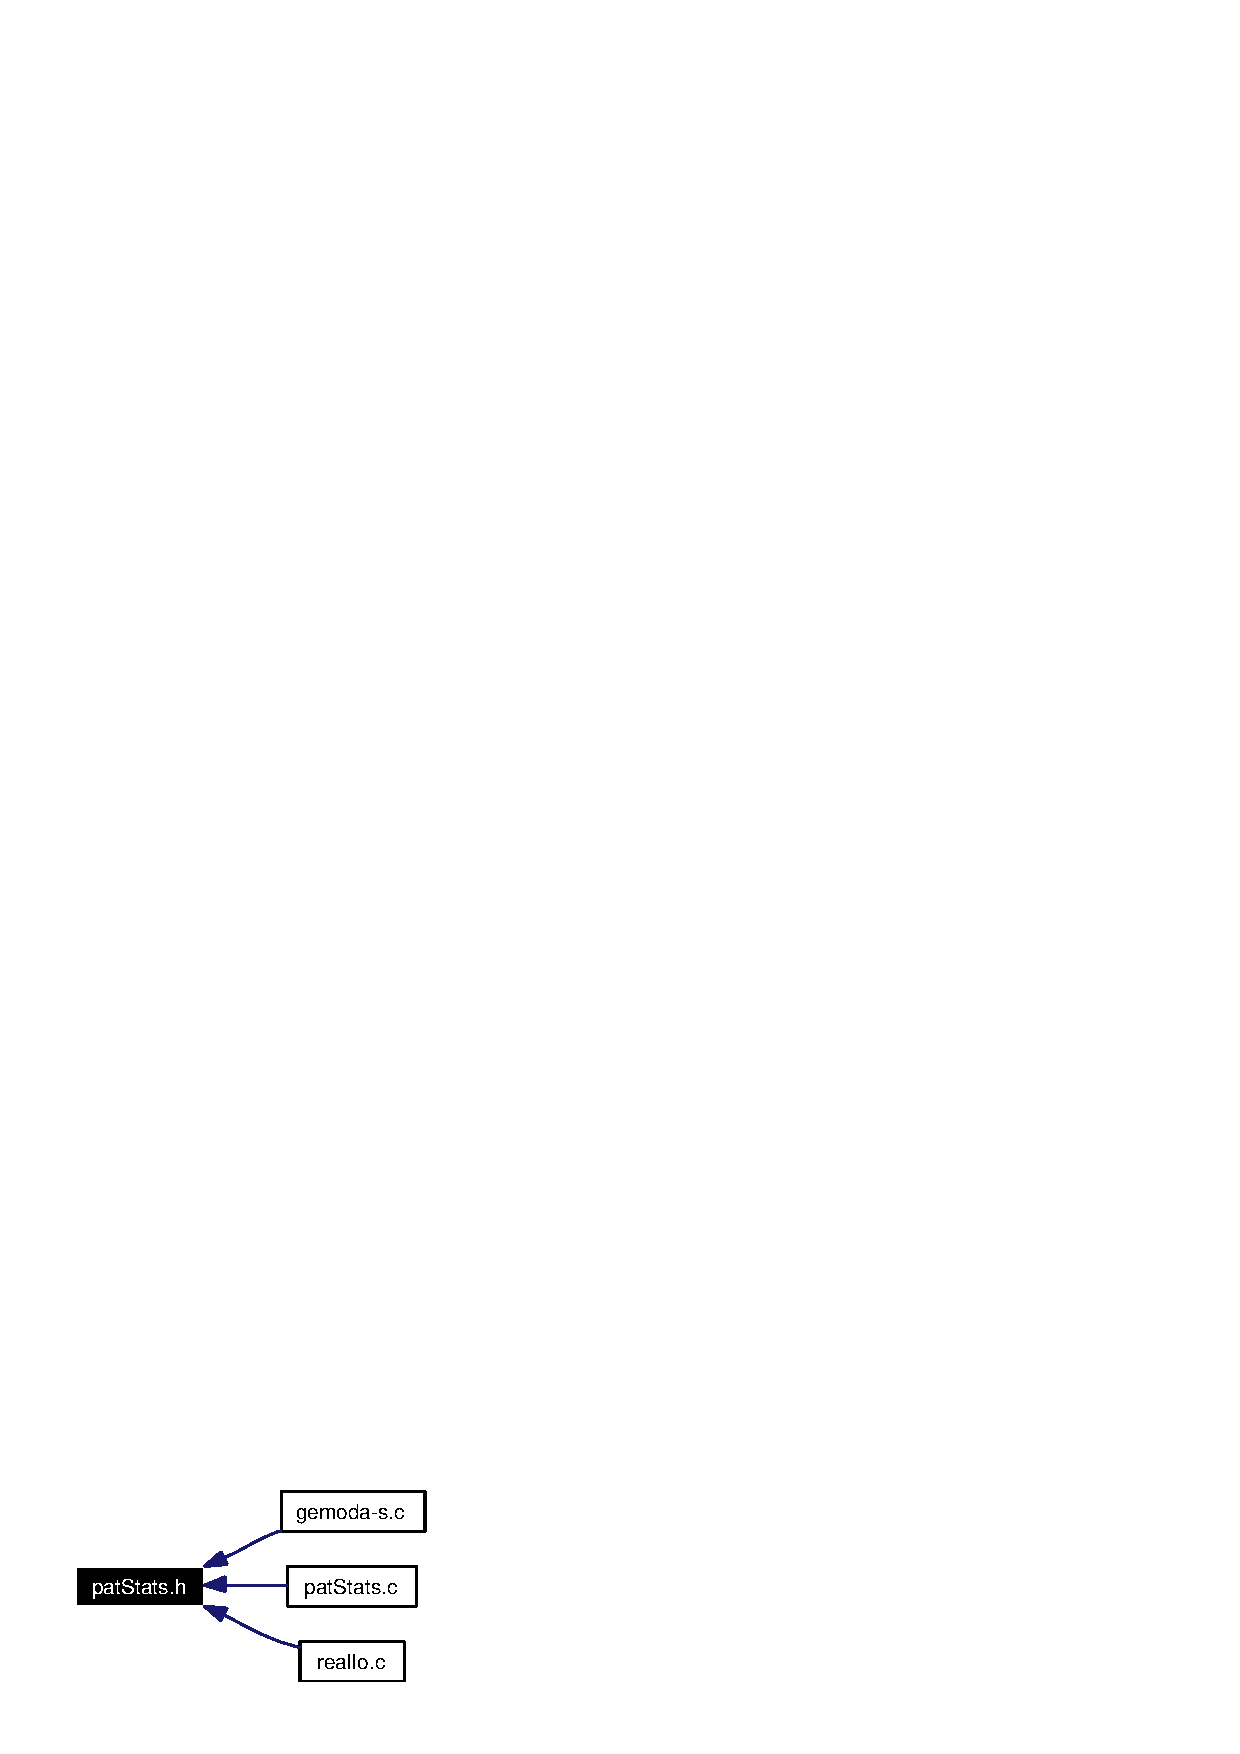
\includegraphics[width=102pt]{patStats_8h__dep__incl}
\end{center}
\end{figure}
\subsection*{Functions}
\begin{CompactItemize}
\item 
unsigned int $\ast$$\ast$ \hyperlink{patStats_8h_a0}{get\-Stat\-Mat} (\hyperlink{structbitGraph__t}{bit\-Graph\_\-t} $\ast$bg, int support, int length, int $\ast$support\-Dim, int $\ast$length\-Dim, int num\-Blanks, int s, FILE $\ast$OUTPUT\_\-FILE)
\item 
int \hyperlink{patStats_8h_a1}{cum\-DMatrix} (unsigned int $\ast$$\ast$d, \hyperlink{structcnode}{cll\_\-t} $\ast$cliqs, int curr\-Support, int curr\-Length, int bg\-Size, int num\-Seqs)
\item 
int \hyperlink{patStats_8h_a2}{calc\-Stat\-All\-Cliqs} (unsigned int $\ast$$\ast$d, \hyperlink{structcnode}{cll\_\-t} $\ast$all\-Cliqs, int num\-Windows)
\item 
\hyperlink{structcnode}{cll\_\-t} $\ast$ \hyperlink{patStats_8h_a3}{sort\-By\-Stats} (\hyperlink{structcnode}{cll\_\-t} $\ast$all\-Cliqs)
\item 
int \hyperlink{patStats_8h_a4}{free\-D} (unsigned int $\ast$$\ast$d, int support\-Dim)
\end{CompactItemize}


\subsection*{Function Documentation}
\hypertarget{patStats_8h_a2}{
\index{patStats.h@{pat\-Stats.h}!calcStatAllCliqs@{calcStatAllCliqs}}
\index{calcStatAllCliqs@{calcStatAllCliqs}!patStats.h@{pat\-Stats.h}}
\subsubsection[calcStatAllCliqs]{\setlength{\rightskip}{0pt plus 5cm}int calc\-Stat\-All\-Cliqs (unsigned int $\ast$$\ast$ {\em d}, \hyperlink{structcnode}{cll\_\-t} $\ast$ {\em all\-Cliqs}, int {\em num\-Windows})}}
\label{patStats_8h_a2}




Definition at line 623 of file pat\-Stats.c.

References calc\-Stat\-Cliq(), cnode::next, and cnode::stat.

Referenced by main().



\hypertarget{patStats_8h_a1}{
\index{patStats.h@{pat\-Stats.h}!cumDMatrix@{cumDMatrix}}
\index{cumDMatrix@{cumDMatrix}!patStats.h@{pat\-Stats.h}}
\subsubsection[cumDMatrix]{\setlength{\rightskip}{0pt plus 5cm}int cum\-DMatrix (unsigned int $\ast$$\ast$ {\em d}, \hyperlink{structcnode}{cll\_\-t} $\ast$ {\em cliqs}, int {\em curr\-Support}, int {\em curr\-Length}, int {\em bg\-Size}, int {\em num\-Seqs})}}
\label{patStats_8h_a1}




Definition at line 460 of file pat\-Stats.c.

References get\-Largest\-Length(), and get\-Largest\-Support().

Referenced by main().



\hypertarget{patStats_8h_a4}{
\index{patStats.h@{pat\-Stats.h}!freeD@{freeD}}
\index{freeD@{freeD}!patStats.h@{pat\-Stats.h}}
\subsubsection[freeD]{\setlength{\rightskip}{0pt plus 5cm}int free\-D (unsigned int $\ast$$\ast$ {\em d}, int {\em support\-Dim})}}
\label{patStats_8h_a4}




Definition at line 637 of file pat\-Stats.c.

Referenced by main().



\hypertarget{patStats_8h_a0}{
\index{patStats.h@{pat\-Stats.h}!getStatMat@{getStatMat}}
\index{getStatMat@{getStatMat}!patStats.h@{pat\-Stats.h}}
\subsubsection[getStatMat]{\setlength{\rightskip}{0pt plus 5cm}unsigned int$\ast$$\ast$ get\-Stat\-Mat (\hyperlink{structbitGraph__t}{bit\-Graph\_\-t} $\ast$ {\em bg}, int {\em support}, int {\em length}, int $\ast$ {\em support\-Dim}, int $\ast$ {\em length\-Dim}, int {\em num\-Blanks}, int {\em s}, FILE $\ast$ {\em OUTPUT\_\-FILE})}}
\label{patStats_8h_a0}




Definition at line 289 of file pat\-Stats.c.

References bit\-Graph\-Row\-Intersection(), check\-Bit(), count\-Set(), delete\-Bit\-Set(), bit\-Graph\_\-t::graph, increase\-Mem(), measure\-Diagonal(), new\-Bit\-Set(), next\-Bit\-Bit\-Set(), and bit\-Graph\_\-t::size.

Referenced by main().



\hypertarget{patStats_8h_a3}{
\index{patStats.h@{pat\-Stats.h}!sortByStats@{sortByStats}}
\index{sortByStats@{sortByStats}!patStats.h@{pat\-Stats.h}}
\subsubsection[sortByStats]{\setlength{\rightskip}{0pt plus 5cm}\hyperlink{structcnode}{cll\_\-t}$\ast$ sort\-By\-Stats (\hyperlink{structcnode}{cll\_\-t} $\ast$ {\em all\-Cliqs})}}
\label{patStats_8h_a3}


This function is used to sort a link to list of cliques by the statistical significance of the motifs found in that linked list.

Definition at line 674 of file pat\-Stats.c.

References cnode::id.

Referenced by main().



